% \paragraph{Introduction}
\section*{To what extent can a wearable robot aid a patient who has lost motor skills?}

Inspired by nature, engineers are moving away from rigid robotics, and towards compliant, \textit{soft robotics}.
Traditional robots with rigid joints allow for high efficiency in single tasks at the cost of reduced interfacing between user and machine \citep{DanielaRus2015Dfac}.
On the other hand, dealing with the particular demands of an individual's disabilities requires high adaptability. These usually are, amongst others, prostheses, surgical and assistive devices, and wearable robots \citep{CianchettiMatteo2018Baos}.
In particular, we explore the latter: exoskeleton gloves which wrap around the user's hand, and aim to support basic functions -- such as grasping and pinching -- which may have been partially or totally lost.

\paragraph{Soft robots imitating life}
\

The progressive iteration of this technology has largely focused on the materials and the mechanism for actuation \citep{ShahidTalha2018MtSR,YeoJooChuan2016SRFS}, ranging from finger-strengthening orthotics to cable-driven gloves (with a supporting backpack) to fluid-actuated gloves \citep{CianchettiMatteo2018Baos,DelphMichaelA2013Asre}, each with an equally as diverse technical challenge, but ultimately with the same goal: to provide adaptable rehabilitation and assistance.
We focus on one such iteration, Exo-Glove Poly, a tendon-driven glove which presents some very interesting concerns, among them ease of use and the quality of the biomimicry, the imitation of nature \citep{KangB.B2012Ftij}.

While some seemingly simple design choices were only recently tackled, such as replacing textiles with washable plastics for easy sanitisation \citep{KangB.B2016IIC}, the operational mechanism is itself an-going challenge.
The gloves work analogously to fingers: non-stretchable cables (tendons) are fixed to the phalanges, the bones in the hand, and link to a small motor on the wrist, in a sort of pulley system that establishes the tension that is needed (See Figure \ref{fig:Wearable_Glove}).
Both the use of cables and the fixation present issues -- the former due to energy losses between the motor and the actuation, and the latter because variations in hand size mean a bad positioning of the ``tendons'' and consequent loss in finger displacement \citep{CianchettiMatteo2018Baos,InHyunki2011Jsau,KangB.B2012Ftij}.

\begin{figure}
    \centering
    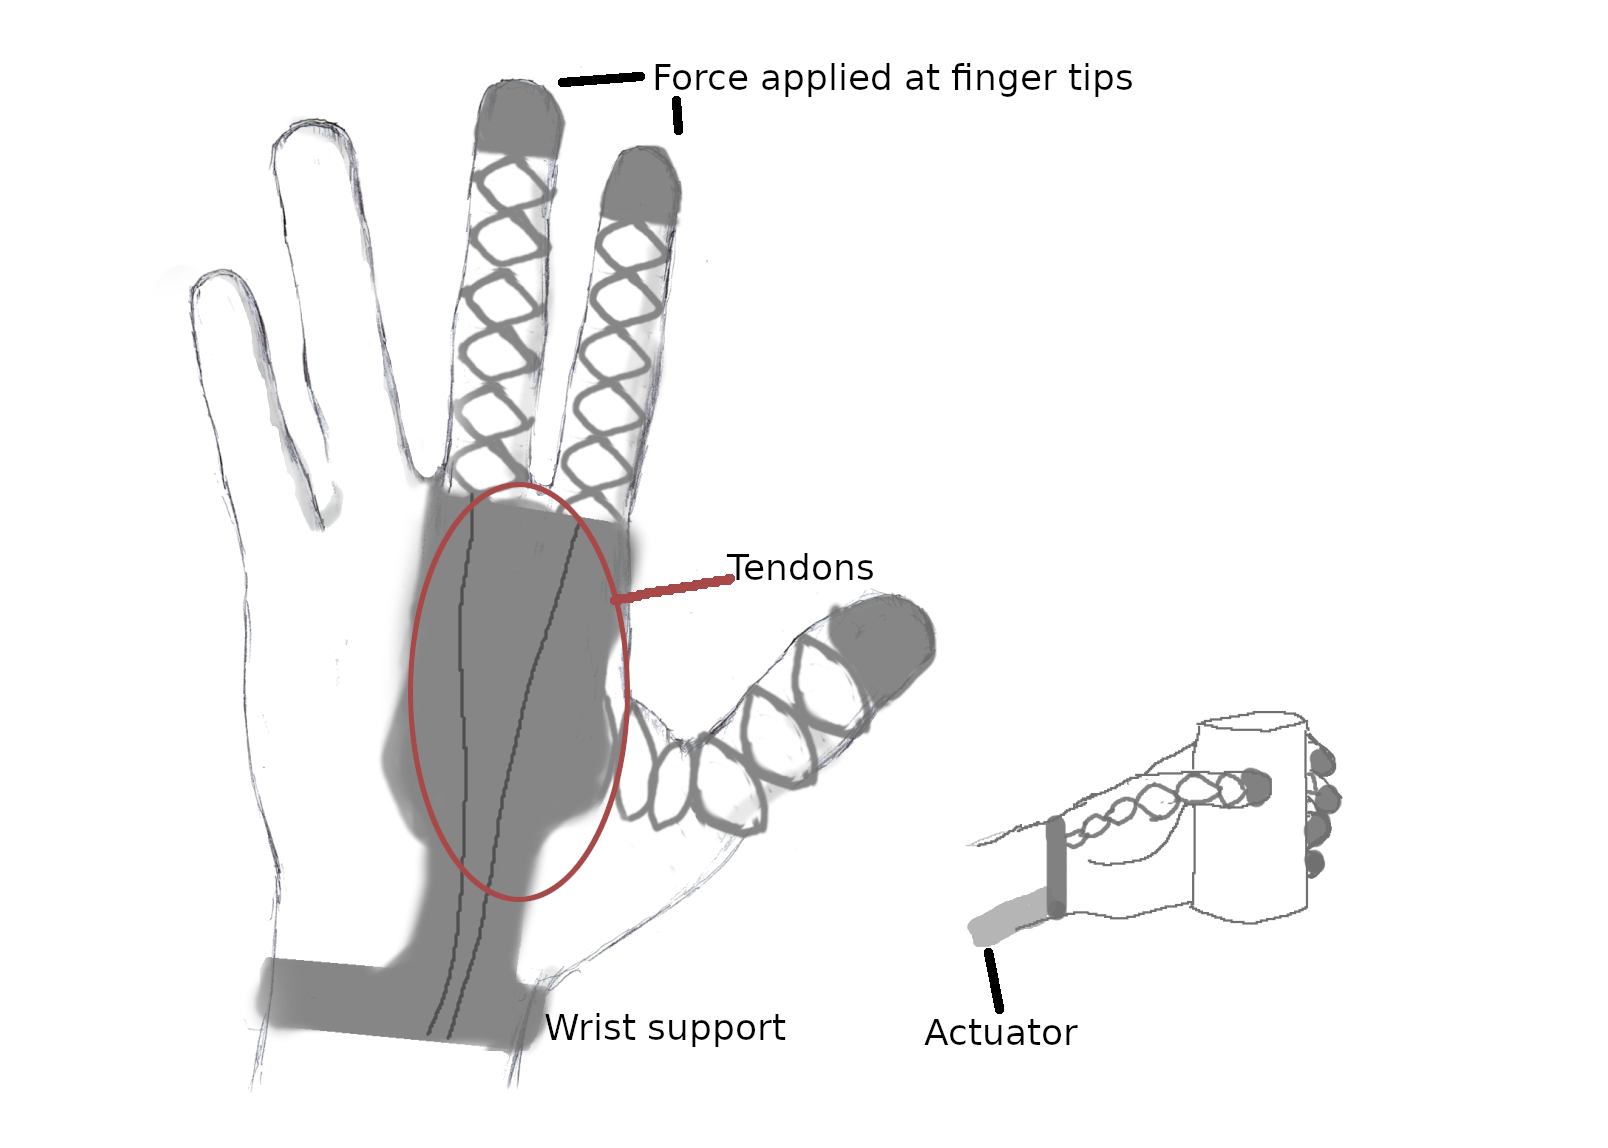
\includegraphics[width=0.8\columnwidth]{files/Gloves.png}
    \caption{Wearable soft robot based on In's 2011 design \citep{InHyunki2011Jsau}. }
    \label{fig:Wearable_Glove}
\end{figure}

% \paragraph{Competing solutions}
Given that researchers in the field are generally focused on variants for specialised applications, it is unsurprising that competing solutions have very diverse audiences and approaches.
One such case called PneuGlove utilises pneumatic actuators -- that is, a compressed air driving mechanism -- for improved hand opening and coordination.
It is an interesting alternative because it is designed for occupational therapy use, strengthening pinching and perhaps training finger individuation \citep{CianchettiMatteo2018Baos,ConnellyLauri2010APGa}, unlike Exo-Glove Poly which simply attempts to support the gross motions.
This is combined with a virtual reality environment that confers a game-like feel to the therapy, generally being well received by patients \citep{ConnellyLauri2010APGa} -- an idea that can realistically be applied to most similar solutions for a higher level of independent training.

Given that most used polymers suffer from deformation, one area explored by new solutions is that of materials -- especially with the use of elastomers, or elastic plastics. 
Amongst them, composites of carbon nanotubes for better strain sensing and gold \& silicone composite for better pressure sensing \citep{YeoJooChuan2016SRFS}.
A particular challenge that Exo-Glove Poly faces is that its mechanism is activated with a button, and so a future solution being sought is the possibility to wear them in each hand, and detect two-handed tasks \citep{SNUBioRobotics2016}.

\paragraph{Conclusion}
\

Wearable soft robots -- and in particular exoskeleton gloves -- present a very interesting tool to increase the level of independence experienced by a person with partial or total loss of manual motor skills.
There is a plenty of variety in how they are actuated, from cables to pneumatics, whether it assists therapy or simply supports motion, and much more.
Considering how emergent these technologies are, a lot of it is focused not only on the mechanics, but also finding the right materials -- whether it can be sanitised, won't cause rashes, is cost-effective to produce, is adaptable to different individuals, is affordable, etc.
One particularly interesting example discussed is the Exo-Glove Poly, a supportive glove aimed at improving grasping and pinching strengths.
While not commercially available, it has taken great strides in the right direction -- providing much needed support and independence who most need it. 